\documentclass[12pt,oneside,a4paper]{article}
\special{papersize=8.5in,11in} % for A4-default configurations on servers
\usepackage{blindtext}
\usepackage{setspace}
\usepackage[left=1.5in, right=1in, top=1in, bottom=1in]{geometry}
\usepackage{graphicx} %TO include graphics in document
\usepackage{amssymb}
\usepackage{algorithm}% http://ctan.org/pkg/algorithms
\usepackage{algpseudocode}% http://ctan.org/pkg/algorithmicx
\usepackage{cite}
\usepackage{pdfpages} % To include title page pdf
\usepackage{url} %For .bib i.e. bibliography
\urlstyle{same} %Keep same font for url in biblography

\begin{document}
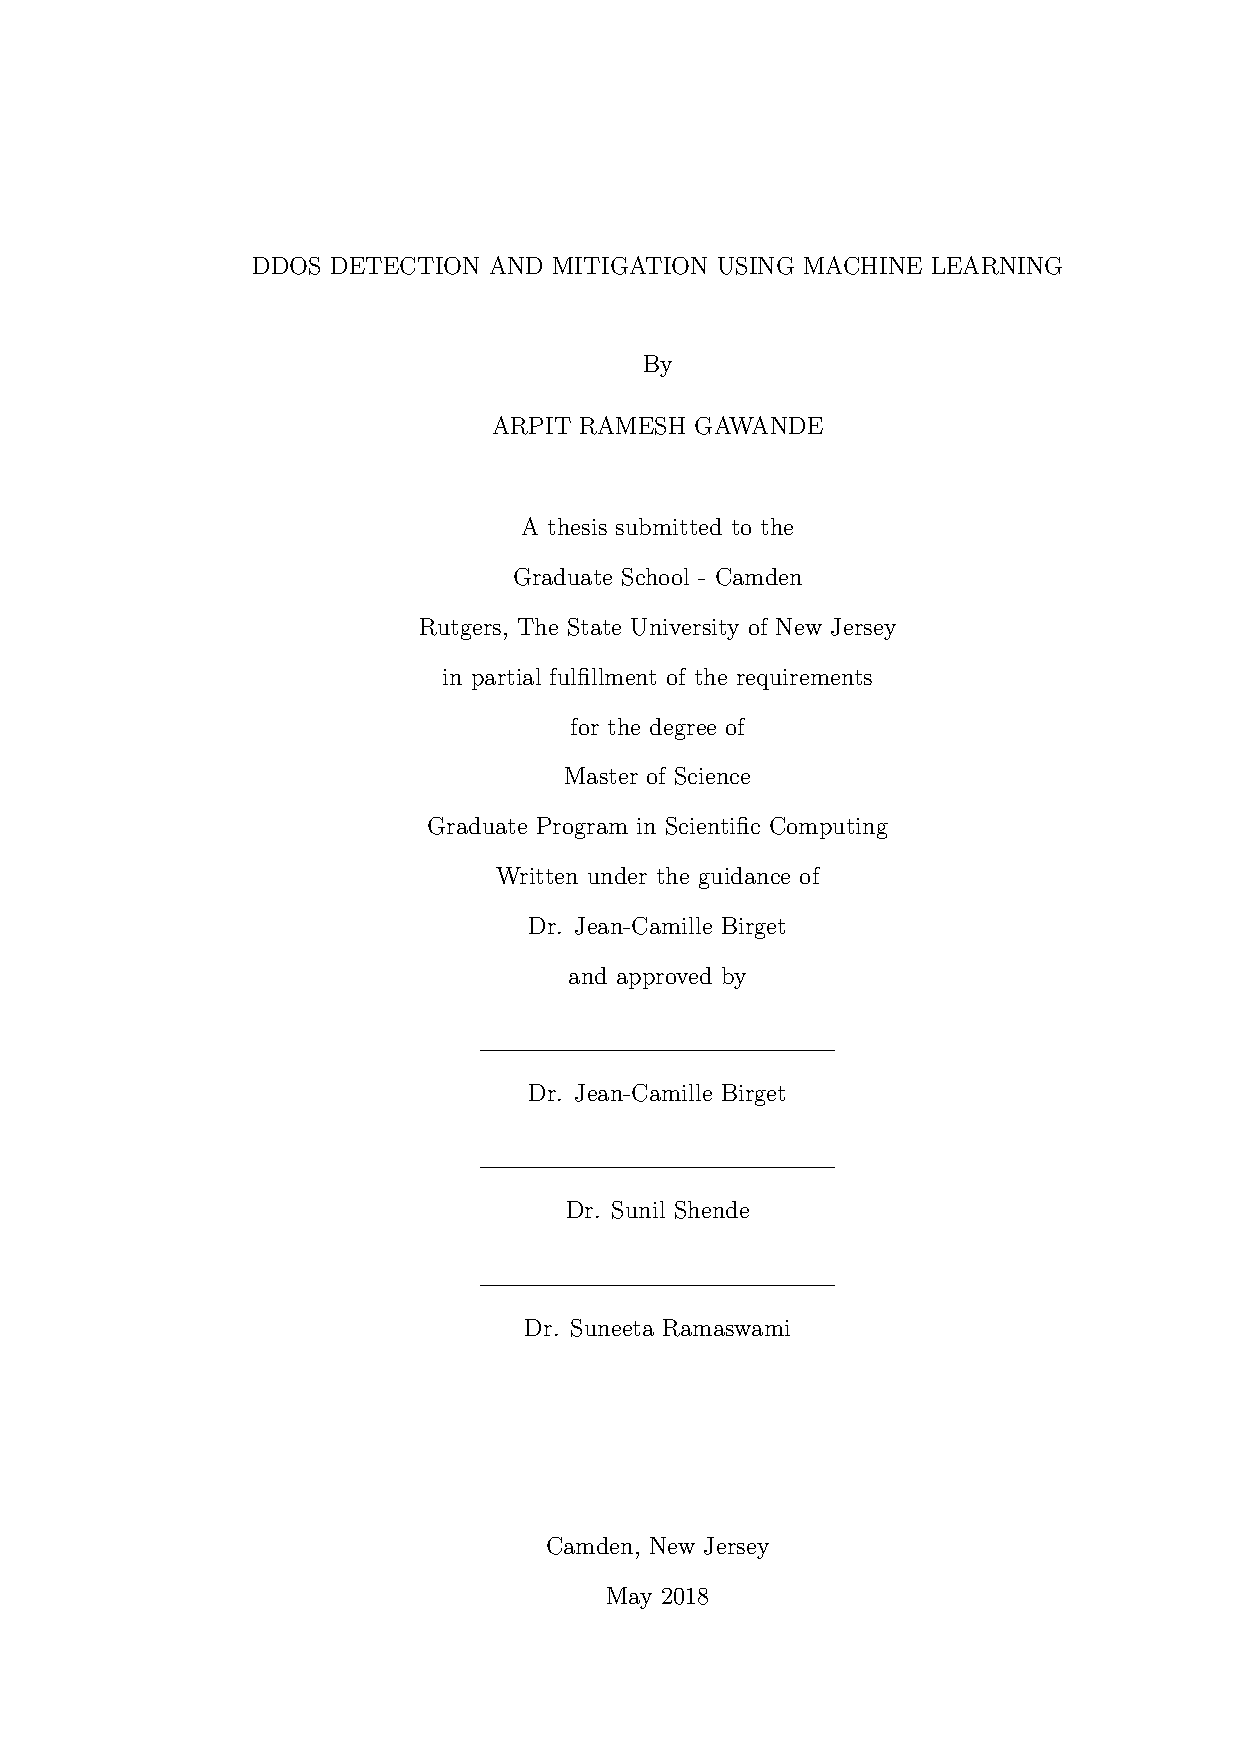
\includepdf{title}
\doublespacing
\renewcommand{\thepage}{\roman{page}}% Roman numerals for page counter
\setcounter{page}{2}% Start page number with 2
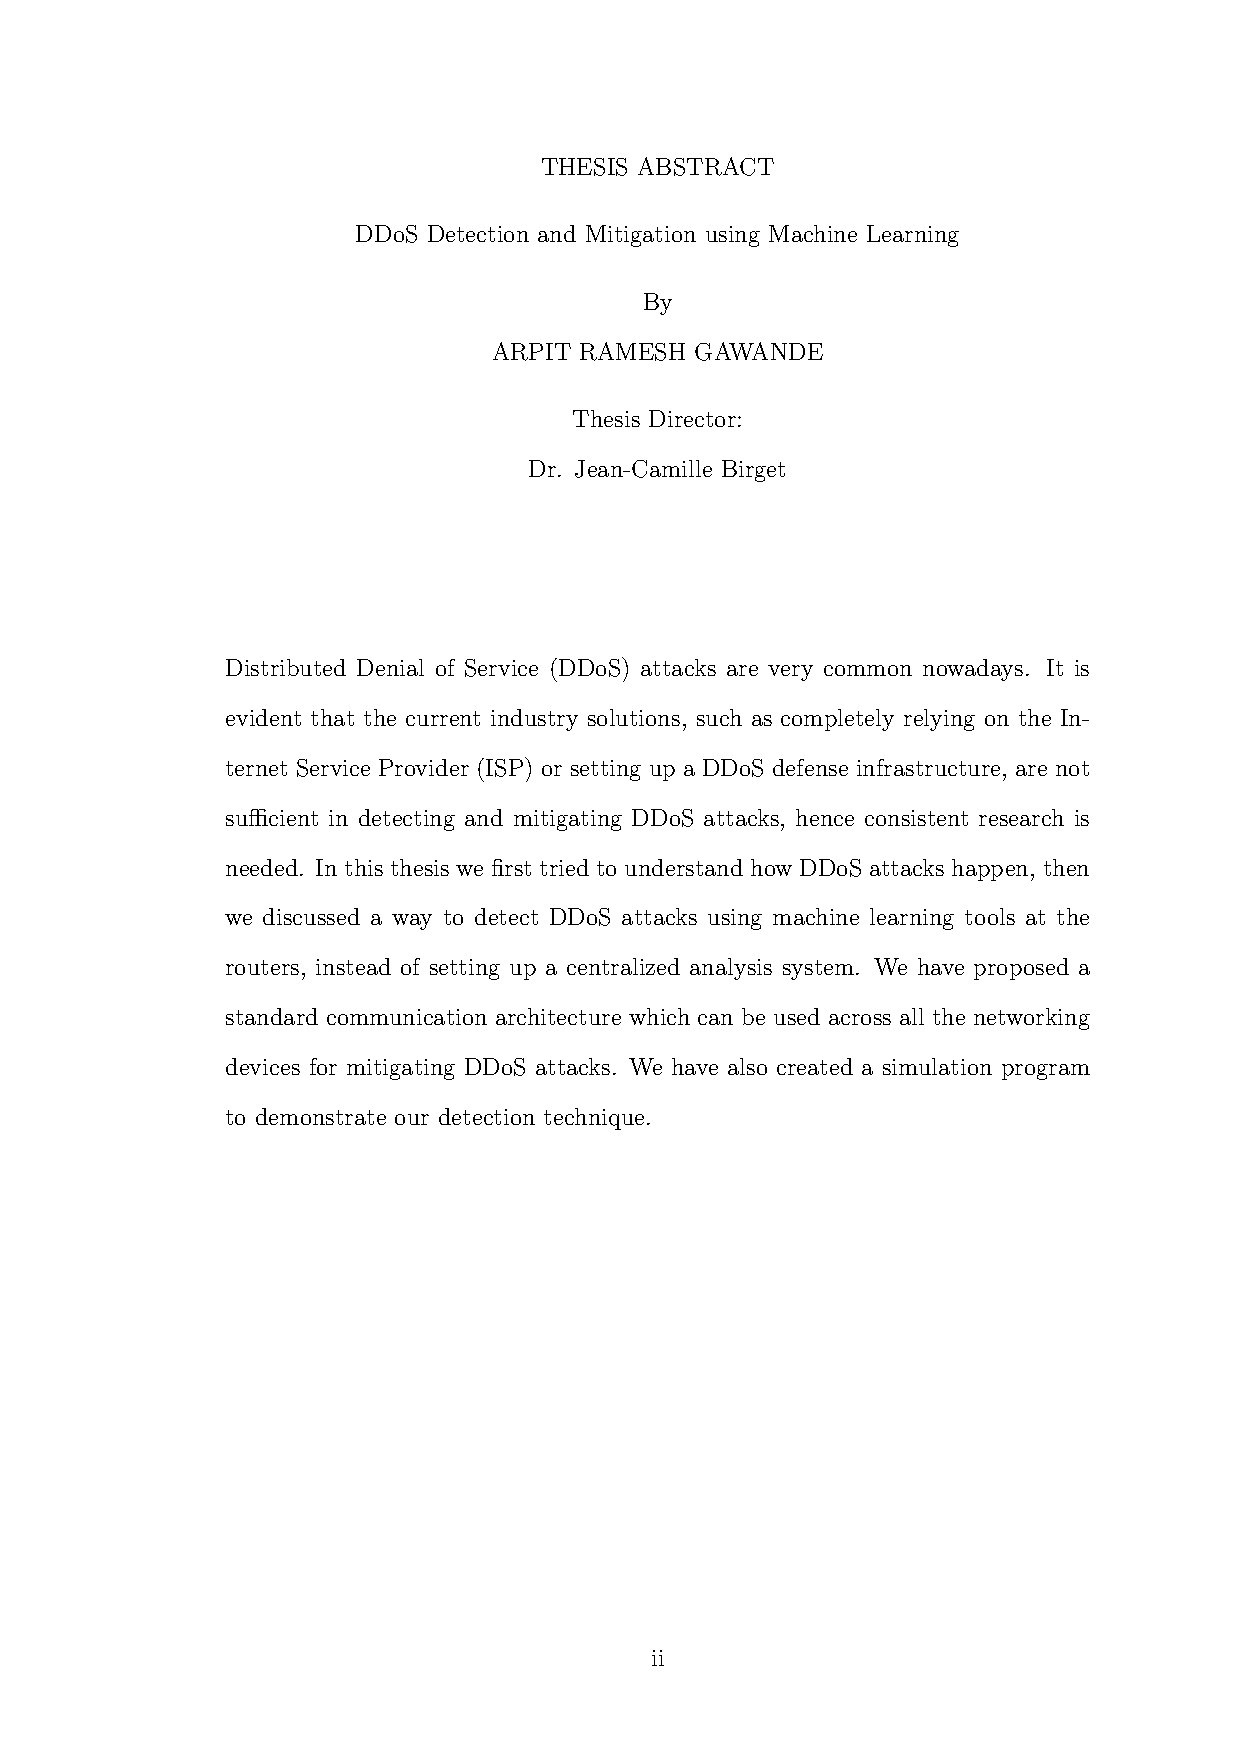
\includepdf{abstract}
\tableofcontents
\newpage
%For page numbering at top right of the page
\pagestyle{myheadings}

\pagebreak
\renewcommand{\thepage}{\arabic{page}}% Arabic numerals for page counter
\setcounter{page}{1}% Start page number with 2

\section{Understanding a DDoS attack}

\subsection{What is a DDoS attack?}
A Distributed Denial of Service (DDoS) attack is a way to jam a host network or its resources with a large number of data packets\footnote{A messages sent on the Internet is broken into shorter messages for transmission. These short messages are called packets. Packet term was coined by Donald Watts Davies.} \cite{network-data-packet} ---or connections, so that the host becomes disabled. There are different types of DDoS attacks such as:
1. Volume-based, e.g., SYN Flood Attacks, in which the victim is flooded with a high volume of  Transmission Control Protocol (TCP)/ User Datagram Protocol (UDP) packets or connections.
2. Application-based, in which an application such as Domain Name Service (DNS), Voice over Internet Protocol (VoIP), or Hypertext Transfer Protocol (HTTP) are attacked.
3. Low-rate, in which the attacker exploits a vulnerability in the application design, e.g., Slowloris.
\cite{DDoS-attacks}

\subsection{Challenges in dealing with a DDoS attack}
Many DDoS attacks happen every day\cite{ddos-attack-news}. Some are reported on the news, while many remain unnoticed. The real challenge in detecting and defending the DDoS attack is its dynamic nature. The source\footnote{The source is a system/device on the Internet that has an IP address and that is under a DDoS attack} is not just a single node or a system on the Internet. There can be many systems participating in a DDoS attack, and often these systems are distributed over different regions of the Internet. Also, the source of the packet is often spoofed\footnote{Spoofing is the way to change the source IP address of the message. This is a known issue in the protocol itself, not in the implementation}\cite{ip-spoofing}. The original attack source is changed in a spoofed data packet, which makes it harder to know the actual IP address of the system from where the attack has originated. In addition, oftentimes the source system itself is not aware that it is compromised, and it's being used as a bot\cite{bot} by an attacker to launch a DDoS attack.

As the source address can't be a reliable way of knowing the attack source (because of spoofing), detecting and mitigating an attack at the destination\footnote{System under a DDoS attack} is not very useful. The destination may know that the attack is happening but to stop it happening it will have to block all the incoming traffic, including the legitimate traffic. To avoid blocking legitimate traffic, companies, such as Cisco and Netgear have come up with some solutions. Many of the solutions provided by these giants---like most of the research that is done in this field---is focused on collecting network traffic flow information\cite{network-traffic-flow} at routers (i.e., gateways). A flow consists of several Internet packets captured during a fixed time interval. The router sends that captured flow information to the central system for analysis. The central system is a hardware and software infrastructure which is capable of processing and analyzing large flow information.\par

Internet Protocol Flow Information Export (IPFIX) protocol created by the Internet Engineering Task Force (IETF), NetFlow protocol created by Ciscos\cite{cisco-netflow}, and Sflow (Sampled flow)\cite{sflow}, are some of the major protocols which are widely used for flow collection and analysis. These protocols define a standard way to export the flow information from a router and similar devices. All these flow monitoring protocols gather information and send the consolidated flow information to the centralized server where the user can login and perform functions; such as, security monitoring, bandwidth monitoring, resource management, traffic analysis, performance management etc. On such systems, there are some modules which are specifically used for anomaly/DDoS attack detection.\par

For example, Cisco netflow has a flow exporter, flow collector, and analysis modules. Flow exporter modules are installed on the routers. The routers, which have flow exporter module, send flow information to the collector module installed on the server. Along with the collector module, the server also has an analysis module, which can be used to detect different patterns in the flow.\par

These technologies scale well and can be sufficient to indicate trends in network traffic; however, they have limitations. 1) They are not cross platform, e.g., the router with Sflow protocol won't work with Cisco routers. 2) They involve setting up expensive hardware, which acts as a collector server. 3) The source address is used for flow analysis, which is not reliable due to IP spoofing in the case of a DDoS attack.\par

\subsection{A DDoS attack detection and mitigation}

A DDoS attack can be detected by checking if there is any anomalous behavior in the network traffic, such as, a sudden increase in the number of packets going to a destination. Detection can occur at the server by observing all of the incoming traffic or it can be done by observing all of the outgoing/incoming traffic at the ISP or at every router. The attack can be mitigated if the anomalous packets are blocked from reaching their destination.

From the previous section we know that the router-based flow analysis can be useful for anomaly detection, but it has limitations because of the way it is implemented. We don't want to set up expensive hardware, we want to have a protocol or a system which is compatible with other routers. Also, we don't want a source IP address for detection analysis. If we can come up with a way to detect anomalies in the traffic at the intermediate devices on the Internet---such as routers--and create a communication protocol between routers and the destination server or network, then better decisions regarding regulating the packet flow can be made.

\pagebreak
\section{Network functioning}

A switch creates a network and a router connects those networks. A router links a computer to the Internet through other routers. Routers are the backbone of the network that helps to forward packets from one point to another point on the Internet. Every packet traveling on the Internet goes through a router\cite{router-switch}. A router knows the destination of a packet, hence it could serve as a first point of knowledge about the change in the packet flow information for a destination. Each router has interfaces to which hosts or other networks are connected. So, a router is aware to what it is connected. It uses protocols to communicate among other routers and by that it gathers knowledge about other routers on the Internet.  Internet Control Message Protocol (ICMP)\cite{icmp} is one of the most frequently used protocol by routers for sharing operational information.\par

\begin{figure}[H]
\centering
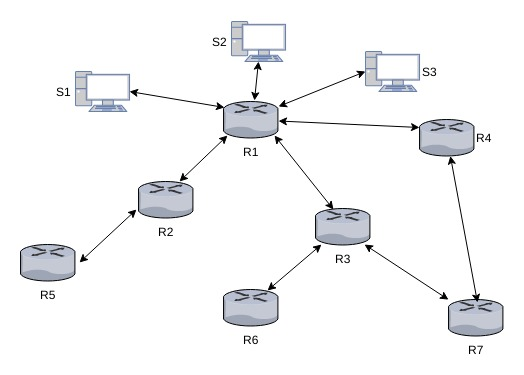
\includegraphics[width=0.70\textwidth]{routers.jpg}
\caption{Network Example} \label{fig:routers}
\end{figure}

Let's illustrate this using an example. In the above figure we can see that hosts S1, S2, and S3 are connected to router R1. Router R1 is connected to the Internet through router R2, R3, and R4, thus every packet traveling to system S2 is coming from either of these three routers. All three routers are located in different geographical regions. Most of the websites are regionally-based, either by county, state, or nation (if we exclude global websites), and hence they are mostly accessed from those regions.\par

Using traceroute tool we can see how many hops\footnote{Hops are intermediate routers in the communication channel} away the destination is. Following is one of the captured route for the Rutgers University website.\par
%\vspace{5mm} % vertical space
\begin{figure}[H]
\centering
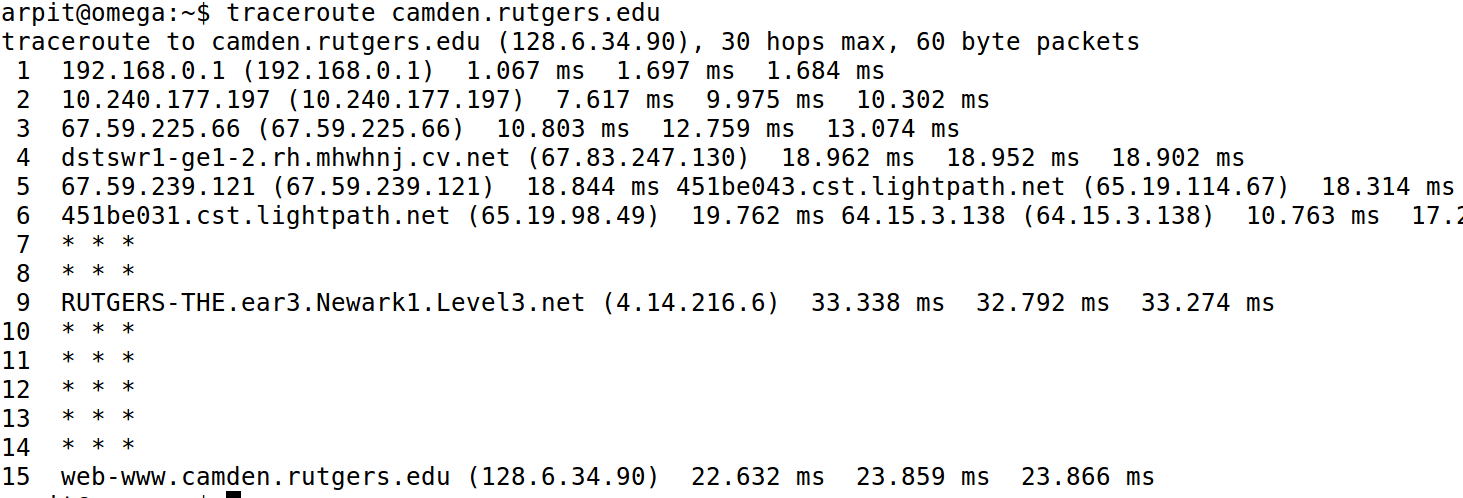
\includegraphics[width=0.90\textwidth]{TraceRoute.png}
\caption{Trace Route: All the routers in the path to destination} \label{fig:traceroute}
\end{figure}

We can see that the packet traveled through 15 routers to reach camden.rutgers.edu server. This route information is found from a location in New Jersey.\par
\pagebreak
\section{Our approach}

\subsection{The router as a point of analysis}
From Figure \ref{fig:routers} and \ref{fig:traceroute} we know that routers are located at different geographical locations and also there are specific regions from which a given website or web server is accessed (with a few exceptions). To know the locations from where the web server/site has been accessed we can use services, called GeoIP services. These services can detect the geographical location of the system from where the IP-packet has originated, but that is just an approximation, based on the source IP and is not always correct. In the case of a DDoS attack, this information is unreliable because the packet source address is often spoofed, hence it's difficult to know the actual geographical location from which the packet has come. If the router through which that packet has traveled can provide its own geographical information, then such information can be useful to understand the path through which the packet has traveled and thus we know the region from where the packet originated.\par

Also, in a normal scenario, there is a consistency in which a website is accessed from different geographical regions, and this consistency can be found by measuring the features, e.g., number of packets that traveled from a router to a destination server. This behavior, i.e., the consistency in which different feature appears in the traffic, can be learned over time. Thus, learning this behavior in the traffic at the router can form the basis of analysis in this thesis. For learning the behavior we will be using the k-means clustering and the one-class SVM classifier algorithms (we are going to explain both these algorithms in detail in coming sections). If there is a significant deviation from the learned behavior of the traffic (i.e., packet flow) to a particular destination then that can be considered as DDoS attack, and that traffic can be bloked at the router. The change in behavior, as well as router geographical region information can also be communicated to the destination which is under a DDoS attack. The destination, on receiving that information, can decide whether it wants the reporting router to discard or forward the traffic for it. This is a selective process in which traffic from only a specific routers is blocked while traffic from other routers remains unaffected.

\begin{figure}[H]
\centering
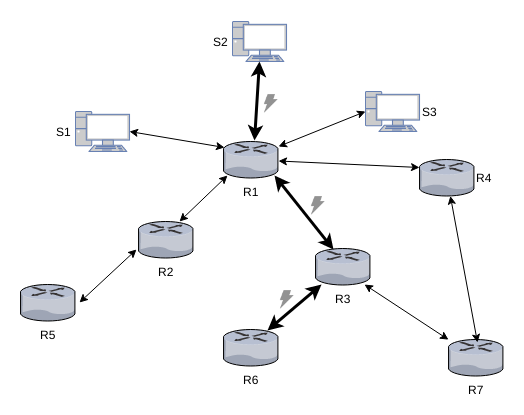
\includegraphics[width=0.70\textwidth]{attack_path.png}
\caption{DDoS Attack path} \label{fig:attackpath}
\end{figure}


In the above figure an attack is initiated from the region where router R6 is located and, from router R6 data packets traveled to the victim\footnote{Victim is a computer system which is under a DDoS attack} system S2. Attack packets traveled through routers R3 and R1 to reach system S2. If we can detect an attack at router R6, then router R6 can discard all the packets heading towards system S2. In this process, only the traffic from router R6 is affected, while traffic from all other routers remain unaffected.

With the advance of electronics and the Internet of Things, processing speed and storage capacity of electronic devices have increased. Routers are no exception; however, storage capacity is always significantly less compared to servers which collect flow data for network traffic analysis. If we use learning techniques that don't need much storage, then we don't have to store large chunk of packets on the router. Instead of storing large chunk of data gather over a longer periods of time for the analysis, we can learn from a relatively small chunk of packets and then discard those packets once the learning is done, leaving behind only the learned information on the router. This is necessary because the number of entries on the Internet routing table has steadily grown. The table has passed 500,000 routes\cite{routing-tablesize}, so storing each and every packet information for all the routes for a longer period of time could be difficult.\par

\subsection{Internet packet flow capturing at the router}

To do the analysis we have to first gather the flow information within a time window (e.g., 300 seconds) which will be fixed at the beginning. Thus, a flow will contain all the packets that are traveled from a router to different destinations during a time span of 300 seconds. We can also combine such flows to form a new flow with larger time windows. For example, if we combine two flows of 300 seconds then we will have a flow of 600 seconds. This flow information can be captured during a particular period or throughout the day. Once we have a flow information, we can apply learning techniques on each flow iteratively to gain deeper knowledge about normal behavior of the flow. For example, an average, how many packets of different protocols are traveling to a given destination from a given router/region during a particular time of the day.

\begin{figure}[H]
\centering
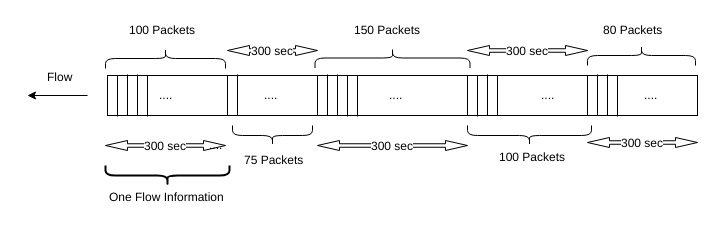
\includegraphics[width=0.90\textwidth]{Data_Flow_Capture.png}
\caption{A 300 second time segment corresponds to a flow of information. The number of packets can vary in a flow.} \label{fig:flow}
\end{figure}

\subsection{Analysis technique}
In the proposed system, each router will itself act as an analyzer. An Internet traffic will be captured on a router. The captured traffic will then be analyzed and features will be extracted from it. Features will be based on the destination IP address (e.g., how many packets of different protocols are observed traveling to a given destination). The extracted features will be used for training a learning algorithm. A learning algorithm creates a model which can be used to predict the behavior of a traffic for a destination. If at any moment in time, the predicted behavior of a traffic for a destination does not match with the actual behavior, then we can say that the destination is under a DDoS attack.

A router will constantly keep learning and updating the learned parameters for different time windows. This window could be any time span in a day, a week, or a month. Before learning from a traffic for a destination, we will use previous learned information to verify that the current traffic for a destination is not an attack traffic.

\pagebreak

\section{Implementation} \label{sec:Implementation}

As discussed previously, there are different types of DDoS attacks, such as volume-based, application-based, and low-rate DDoS attacks. Among these different types of attacks, the volume-based attack is the most common. In a volume-based attack a destination server is flooded with a high volume of Internet packets (TCP, UDP, HTTP or ICMP), which makes the server unable to serve the requests.

To demonstrate the suggested approach, we simulated a volume-based attack. In a real world, volume-based attacks are orchestrated using bots. Bot\cite{bot} is computer program designed to perform a particular task and is under the control of an attacker. Bots are installed on a compromised computer systems by an attacker. Bots are not bound by geographical boundaries, they can be anywhere on the Internet. The Internet is a connection of different computer systems communicating with each other through different channels, such as cables, satellite, or radio devices, and these communication channels run throughout the globe. A botnet (i.e. a network of bots) is created by an attacker to launch a DDoS attack.

For our simulation, instead of designing a bot program, we have used Low Orbit Ion Canon(LOIC) tool which is a free DDoS attack launching tool. Even attackers use this tool in the real world to launch a DDoS attacks.

We used Wireshark, an open source tool, for capturing Internet traffic. Wireshark can capture all digital information received or sent through different devices such as Ethernet or Wi-Fi devices. It also helps identify different protocol packets (e.g., TCP, UDP), within the wrapper packet created at Data Link Layer.\par

\begin{figure}[H]
\centering
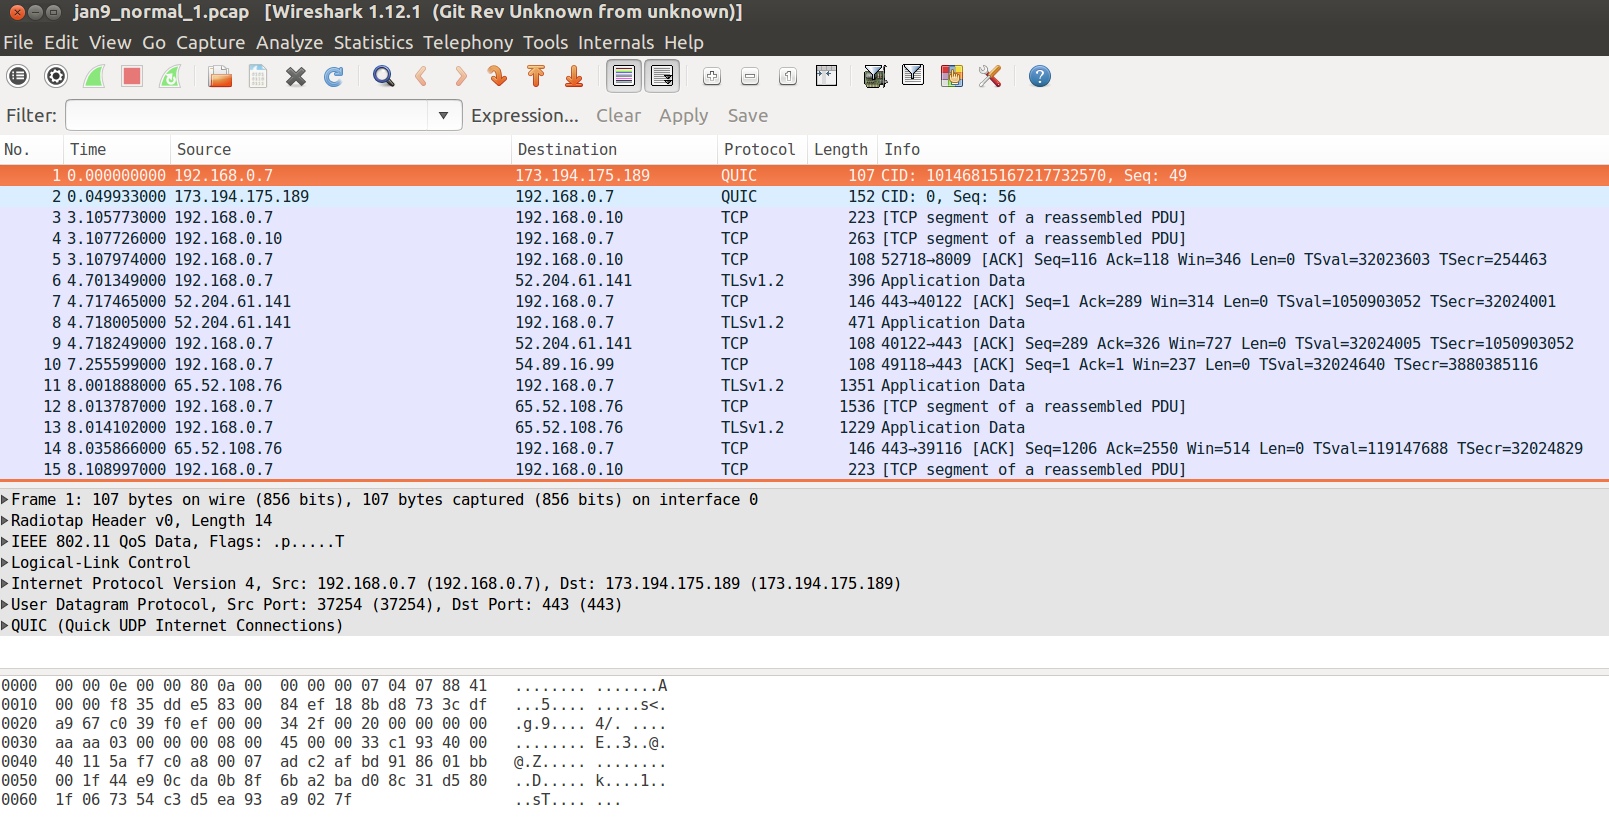
\includegraphics[width=0.90\textwidth]{Wireshark_Tools.png}
\caption{Wireshark Tool: snippet of captured packets} \label{fig:wireshark}
\end{figure}

For the demonstration of our approach, we have created a small network which has one router and a couple of host machines. Each machine can be a victim of a DDoS attack. We installed the Wireshark tool on one of the machine in this network. For capturing traffic in the network, we used Wireshark's Promiscuous mode. In a Promiscuous mode, a network interface can record not only the traffic that it is intended to send-receive, but all the traffic on the network. This allows us to capture all the traffic on the network. This setup is similar to a router on the Internet which captures all the traffic going to different destination through it.

\begin{figure}[H]
\centering
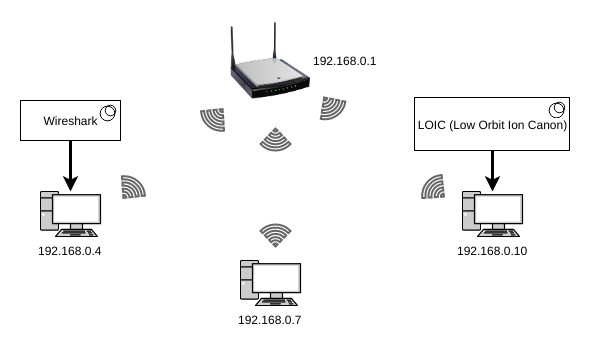
\includegraphics[width=0.90\textwidth]{demo_network.png}
\caption{Network for simulating a DDoS attack detection} \label{fig:demonetwork}
\end{figure}

To capture a normal traffic, we started Wireshark tool and let it run for couple of hours. To capture an attack traffic, we orchestrated a DDoS attack on one of the host (e.g., 192.168.0.7 in Figure \ref{fig:demonetwork}) in our network. This attack was engineered using the LOIC tool that was installed on another host (e.g., 192.168.0.10 in Figure \ref{fig:demonetwork}). This tool allowed us to launch TCP and UDP flood attack on any destination.

All the traffic, including the normal and the attack traffic, was captured using Wireshark. Packets are captured for about five hours in the given network. Once the packets are captured, they were saved as pcapng file, which is a Wireshark file format for captured packets. The packets captured during a normal traffic, and during an attack were saved separately on the file system. The normal traffic information was used for training and testing the learning algorithms (we will explain them in later sections), while an attack traffic was used for detecting an attack. Wireshark captures every detail of a packet, but we didn't need all of the information, we were interested only in the IP layer information of a packet. Most routers analyze only the IP layer information for routing, having said that, there is no reason that information present at other layers of a packet cannot be analyzed. For our demonstration purpose we choose only the IP layer information of a packet.\par

A data extraction program was written in the Python language to extract the IP layer information from a captured packet. This program extracts IP address, port and time information from each captured IP-packet\footnote{A packet containing IP layer information}.

\begin{table}[H]
\centering
  \begin{tabular}{| l | c | l | c |}
    \hline
    Destination IP Address      & Protocol  & Time stamp(Sec.)  & Sample Number \\
    \hline
    52.6.129.72         & 6         & 1512094785.928596000  & 1 \\ \hline
    192.168.0.4         & 6         & 1512094785.946987000  & 1 \\ \hline
    192.168.0.4         & 17        & 1512094786.148488000  & 1 \\ \hline
  \end{tabular}
\caption{Sample file snippet (row represents an IP-packet)} \label{table:sample-file-snippet}
\end{table}

The data extraction program divides the captured traffic into samples. In our case, a sample was a traffic captured during a 300 seconds time window. Samples were stored on a file system for further processing. This sampling of traffic is a continuous process. We then ran another program to extract the flow information from a sample file. A ``flow'' for a destination contains a count of different types of packets captured for a destination in a sample file. This flow represents a ``training example'' for the learning algorithm we used (see Table \ref{table:feature}). Thus, A flow information for a single destination is regarded as a training example and flow information for all the destinations in a sample file regarded as one training set. Each training example is labeled with destination IP address.

\begin{table}[H]
\centering
  \begin{tabular}{| l | c | c | c |}
    \hline
    & \multicolumn{3}{ |c| }{IP-Packet count} \\ \cline{2-4}
    {Destination IP Address}  &ICMP  &TCP &UDP\\
    \hline
    172.217.10.134  & 0     & 8     & 12 \\ \hline
    65.19.96.252    & 5     & 0     & 192 \\ \hline
    68.67.178.134   & 0     & 78    & 0 \\ \hline
  \end{tabular}
\caption{Three training examples represent ``flow'' for three destination addresses} \label{table:feature}
\end{table}

In above figure \ref{table:feature}, ICMP, TCP, and UDP packets count for each destination is calculated during a time window of 300 seconds, so, it's a training set with three training examples. We kept aside few training sets for testing our algorithms.

We trained our algorithms using multiple training sets. After training, a trained model was created, and stored on file system. Sample files were discarded, and new samples were created for further training. This training process has to be continuous process in order to correctly reflect the overall traffic behavior at a router. Every time the new information was learned, it was augmented with the previous learned information, so that we have correct model for a DDoS attack detection. Learning process can be done over the course of a day, a week, a year and so on. We can have separate learning information for the traffic in the morning from 9 a.m. to 12 p.m., and the traffic in the evening 6 p.m. to 12 p.m. Thus, a router will have multiple trained models, one model for one specific time span.

Because an attacker oftentimes uses different ports and employ spoofing technique for a DDoS attack, destination port number and source IP address are not reliable features for detecting a DDoS attack. Packet analyzing is often difficult due to the size and the encryption, while flow based model is more reliable and fast. Due to these reasons, we did not consider features hidden inside the packet (e.g., information available at different layer of a packet), and also did not consider a source IP address or a destination port information for building prediction models.

We used the Python program to create training sets as given in Table \ref{table:feature}. Each row in a training set is one training example with the destination IP address as a label. A training example is $\mathbb{R}^3$ vector whose elements are the number of packets observed for a particular protocol for a destination during a fixed time (e.g., 300 second window). There are around 150 protocols managed and assigned by the Internet Assigned Numbers Authority (IANA), but the most commonly used protocols in a DDoS attack are ICMP, TCP, and UDP. Hence, for the training and analysis purpose we used only these three protocols as the desired features.

Each sample file was processed, and corresponding train and test set was created. Train and test sets were stored on the file systems, so that, they can be used by our programs for training the algorithms and testing the model.

\subsection{Machine learning}

According to Tom Mitchell\cite{machine-learning-def}, a computer program is said to learn from an experience E with respect to some task T and some performance measure P, if its performance on T, as measured by P, improves with experience.

A learning algorithm builds a hypothesis using a training set as an input. The hypothesis is then used to perform predictions. Most common categorization of machine learning algorithms are Supervised and Unsupervised.

Let $f: \mathbb{R}^d \rightarrow \mathbb{R}^d$ be the function that we need to guess from input vectors $x^{1}, x^{2}, ..., x^{n}$, also called as `input variables' or `feature vectors'. Let $\Xi$ be a set of such input vectors. Let $n$ be the number of input vectors in training set $\Xi$. Let $H$ be any set of functions. Let $h:\mathbb{R}^d \rightarrow \mathbb{R}^d \in H$ be the hypothesis about function $f \in H$. We selected $h$ based on training set $X \subseteq \Xi$, of $m$ input vectors. In supervised learning, we know the values of $f$ for $m$ samples, in training set $X$. We assume, if we can find hypothesis $h$ that closely agrees with $f$ for the members of $X$, then this hypothesis will be a good guess for $f$ when $X$ is large. In unsupervised learning, we simply have a training set of vectors without function values for them. The problem in this case, typically, is to partition the training set into subsets, $X_1,.. ,X_{N}$, in some appropriate way.\cite{machine-learning}

A supervised algorithm, such as one-class Support Vector Machine (one-class SVM)\cite{svm}, is efficient in identifying anomalies in a data; however this algorithm is process-and memory-intensive. Training such algorithm for each and every IP address is very costly in terms of resources. So, our approach was to first cluster the IP addresses based on the features using unsupervised learning algorithm, such as k-means, and then applying one-class SVM on the clusters to decide their boundaries. K-means algorithm is fast and consumes fewer resource compared to one-class SVM. This makes it a good first choice for routers (traditionally router has less processing power and less memory).

\subsubsection{Feature scaling}

Before feeding training data acquired in an earlier stage, to a learning algorithm, we had to do feature scaling (which is also called Standardizing). Feature scaling is done by subtracting the mean and scaling the feature to a unit variance value. It's necessary because, different features which are at different scales, could cause one feature to dominate others in the algorithm output result. For example, consider two vectors (1, 2, 3000) and (1, 3, 2000). If we calculate the Euclidean distance between these two vectors using formula $\sqrt{\sum_{i=1}^n (p_i - q_i)^2}$, then the distance is $\sqrt{(1-1)^2 + (2-3)^2 + (3000-2000)^2}$ . This show, the larger term is dominating the resultant distance.

If we consider a training example without a label (i.e., without destination IP address) as a vector, then each coordinate in the vector is a feature. To standardize the vector---mean and standard deviation was calculated for the set of input vectors. Then, a new vector was created by subtracting the mean from each feature vector and dividing that feature vector by its standard deviation. The new vector created after this step was standardized vector. A set of such standardized vectors was used as input to learning algorithms.

\hspace{2cm} Standardization formula: $x' = \frac{x - \bar{x}}{\sigma}$,

where $x$ is a feature vector, ${\bar{x}}$ is the mean and $\sigma$  is its standard deviation.

\subsubsection{Clustering} \label{subsec:Clustering}

A clustering algorithm will take training vectors as input, and then group them with some scheme. K-means\cite{k-means-clustering} clustering is one of the most efficient algorithms for creating clusters. This algorithm initially takes any $k$ randomly chosen points $\mu_{1}, \mu_{2}, ..., \mu_{k}$ (called, ``centroids'' or ``cluster centers''), as a input, from training set $X = \{x^{1}, x^{2}, ..., x^{m}\}$, $x^{i} \in \mathbb{R}^d$, $i= {1,2, ..m}$, and then group elements in training set based on how close they are from the centroid. The centroids are recalculated after every cluster assignment. Following is Lloyd's algorithm. It is the most popular heuristic algorithm for k-means clustering.

\begin{algorithm}[H]
\caption{k-means}\label{k-means}
\begin{algorithmic}[1]
  \State{Random choose any $k$ points $\in X$ as centroids.}
  \Repeat
  \State{Calculate distance for each element (or data point) of the training set to all the centroids.}
  \State{For each element, assign centroid which is nearest to it.}
  \State{Recalculate new centroid for all the elements in one cluster by taking the mean. If ${x^j_1, x^{j_2}, ..., x^{j_n}}$ are the elements of the cluster $j$, then for cluster $j$ new centroid will be $\mu_{j} = \frac{1}{n} [x^{j_1} + x^{j_2} + ... + x^{j_n}]$, where $n$ is the number of points assigned to cluster $j$. Do this for all the clusters.}
  \Until{No data point is reassigned to a different centroid.}
\end{algorithmic}
\end{algorithm}

For this thesis we used k-means++ algorithm. It is an improvement of k-means. In k-means++ algorithm an arbitrarily initialization step is replaced by simple, randomized seeding technique. K-means++ tries to find the centroids as far away from each other. If $D(x)$ is the shortest distance from a data point $x \in X$ to the closest centroid we have already chosen, then following is k-means++ algorithm\cite{k-means++}.

\begin{algorithm}[H]
\caption{k-means++}\label{k-means++}
\begin{algorithmic}[1]
  \State{Select a centroid $\mu_1$, chosen uniformly at random from $X$, as first centroid.}
  \State{Choose a new centroid $\mu_i \in X$, such that the probability $\frac{D(\mu_i)^{2}}{\sum_{x \in X} D(x)^{2}}$ is highest.}
  \State{Repeat Step 2. until all $k$ centroids are taken.}
  \State{Proceed with the Lloyd's k-means algorithm, skipping random initialization stage.}
\end{algorithmic}
\end{algorithm}

For our DDoS attack detection program, we used Scikit-learn libraries. Scikit-learn is most popular and rich open-source machine learning software library for Python programming language, and it has implementation for both k-means++ and one-class SVM machine learning algorithms. It also has data preprocessing programs, such as feature scaling.

We took a training set (in the format given in figure \ref{table:feature}) and we clustered them using k-means++ clustering algorithm from Scikit-learn.

\begin{figure}[H]
\centering
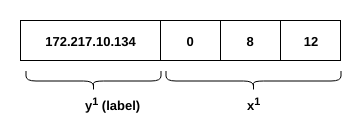
\includegraphics[width=0.70\textwidth]{training_example.png}
\caption{One training example} \label{fig:training_example}
\end{figure}

Before doing clustering, we had to first determine the number of clusters and centroids\footnote{A centroid is a vector which is an arithmetic mean of all the points in a cluster.}. A centroid represents a cluster in a training set. Deciding number of clusters is important, because randomly choosing the number of clusters may not have correct clustering. To find the optimal number of clusters in our training set, we used Elbow method. Elbow method checks the portion of the variance explained by a function of the number of clusters. The cluster number that has produced least variance for the next cluster number was selected as best choice for clustering our training set. The following is an elbow diagram produced using Elbow method. In this diagram, x-axis represents the number of clusters and y-axis represents the variance explained. The cluster number at the ``elbow'' of the diagram is the best choice.

\begin{figure}[H]
\centering
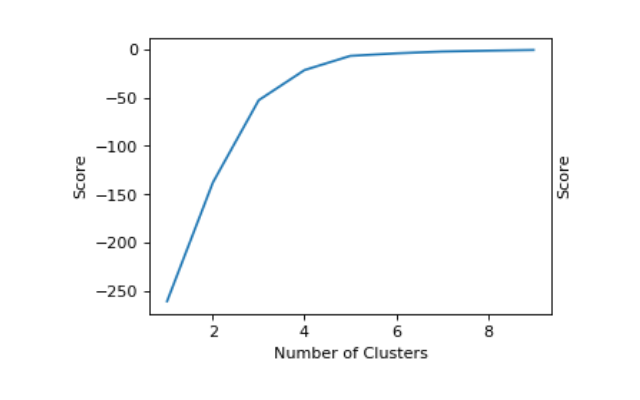
\includegraphics[width=0.70\textwidth]{elbow-method.png}
\caption{Elbow Method for cluster count determination} \label{fig:elbow-method}
\end{figure}

As we had multiple training sets. We first ran k-means++ algorithm on all training sets using the number of clusters found in Elbow method as input. After clustering was done, we got one centroid set for each training set (One centroid in a centroid set represents one cluster in a training set). For our detection technique, we needed only one set of centroids that can correctly cluster the traffic. If we choose $k$ number of clusters for the clustering, then this set will contain $k$ centroids. To determine such centroids (i.e., centroids set), we first removed the outliers among all the centroids (one per training set), and then calculated the median of all the remaining centroids. Such median is a good estimate of all the centroids. These estimated centroids were used for clustering the samples in the future. Following is the example of centroid vectors with two clusters. A row represents a cluster and a column represents a feature.

\begin{table}[H]
\centering
  \begin{tabular}{ l | c  c  c }
    Cluster      & ICMP  & TCP  & UDP \\
    \hline
    0         &{-0.16815612}       &{-0.14928111}    &{-0.16948046} \\
    1         &{-0.18181818}       &{5.13527652}     &{5.68956244} \\
  \end{tabular}
\caption{Example of cluster centroids: A row is a cluster and a column is a feature} \label{table:centroids-example}
\end{table}

The estimated centroids were used to cluster all the training sets and to label each training example with cluster number.

After clustering is done, it needed to be tested for accuracy, i.e., how similar the test set clustering is with training set clustering. This can be done by checking whether or not an IP address has the same cluster number assigned in both the training and the test sets. For measuring this similarity Rand Index(RI)\cite{ri-index} was used. RI is a measure of how well does the test clustering matches with the trained model:

\hspace{4cm} $RI={\frac {TP+TN}{TP+FP+FN+TN}}$,

$TP= true\ positives$, $TN=true\ negatives$, $FP= false\ positives$, and $FN= false\ negatives$

Because training sets contain the flow information for different IP addresses on a router during a fixed time window, there is a very high probability that the same destination IP address is captured in multiple training sets. Our goal was to find correct cluster for each destination IP address. To achieve this goal, we labeled the IP addresses with clusters in which they found most of the time, e.g., if an IP address is labeled with cluster `0' in five training sets and cluster `1' in two training sets, then the IP address was labeled with cluster `0'. We also calculated and stored the total packet count for a destination in a flow.

\begin{table}[H]
\centering
  \begin{tabular}{| l | c | c | c | c |}
    \hline
    {Destination IP Address}  &Cluster  &Packet Count \\
    \hline
    74.125.141.106  & 1     & 113  \\ \hline
    72.30.2.182     & 0     & 16   \\ \hline
    64.94.191.14    & 0     & 22   \\ \hline
  \end{tabular}
\caption{Learned information after clustering} \label{table:learned-clustering}
\end{table}

Clustering information tells us the normal behavior of packets traveling from a router to a destination, i.e., for normal traffic, every time we do clustering, we should expect an IP address to be found in the same cluster it was found during the training. But if there is a DDoS attack on a destination, then the destination IP address can be found in different cluster.

\subsubsection{Anomaly detection using one-class Support Vector Machine} \label{subsec:Anomaly_Detection}

From the experiments on different training sets, we found that the destination under attack is sometime labeled with the same cluster number that we had after training. We had a fixed number of clusters, so the training example for a destination IP address gets assigned to the cluster whose centroid is the nearest (which was the same cluster it was labeled in the training). To avoid such a situation, we had to create boundaries for the clusters. If any IP address was found outside of the cluster boundaries, then traffic for that destination was considered suspicious. This provision made sure that the attack on a destination IP address was detected even if traffic for that destination was assigned to the same cluster it was assigned in the past.

To create cluster boundaries, we used one-class SVM classifier. One-class SVM classifier is used when we have only one type of training examples. It classifies the training examples into one class. In our case, training vectors (also called as data points) in a cluster formed a class. So, for each cluster we had one classifier that classifies whether or not a training example is inside the cluster.

\paragraph{Support Vector Machine (SVM):}

SVM is a supervised learning algorithm which tries to classify training examples into two classes. Classification is based on the labels of a training set.
Consider training set $\{(x^{1},y^{1}), .., (x^{m},y^{m})\}$, where $x^{i} \in \mathbb{R}^d$ is the training example, and $y^{i} \in \{-1, +1\}$ is the label (or a class) for $x^{i}$. SVM will separate these classes using a line or a curve.

SVM tries to create a non-linear separation boundary by projecting data points using a non-linear function $\Phi:x \rightarrow \phi(x)$ (called ``kernel'' trick) to higher dimensional space. The data points in space $I$ which can't be separated by a line are projected to feature space $F \subseteq \mathbb{R}^d$, where, there can be a hyperplane that separates data points of one-class from another. If that separating hyperplane is projected back on the original space $I$ then we get a non-linear curve.\cite{svm}

\begin{figure}[H]
\centering
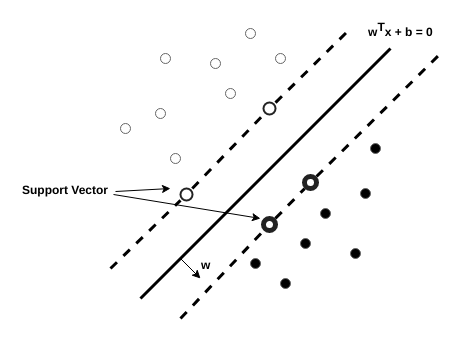
\includegraphics[scale=0.5]{SVM.png}
\caption{Linear Separation using Support Vector} \label{fig:SVM}
\end{figure}

The hyperplane is represented with the equation $w^{T} \phi(x) + b = 0$, where $x \in \mathbb{R}^d$, $w \in F$ and $b \in \mathbb{R}$. This hyperplane separates the training examples labeled with $-1$ and $1$. The position of the hyperplane is such that, the distance from the closest point in each class to the hyperplane is same. To avoid over-fitting, slack variable $\xi^{i}$ is introduced. Over-fitting happens because the learned hypothesis fits training examples so well that it fails to generalize new examples. The SVM classification is an optimization problem stated as follows:\cite{svm} \cite{svm-ml}

\begin{center}
  ${min}_{w,b,\xi^i} \ \frac{||w||^2}{2} + C \sum_{i=1}^m \xi^i$ \\
  $\mbox{ subject to: }$ \\
  $y^i( w^T \phi(x^i) + b) \geq 1 - \xi^i \mbox{ for all } i = 1, \dots, m$ \\
  where $y^{i} \in \{-1, +1\}$, $x \in \mathbb{R}^d$, $b \in \mathbb{R}$ and $\xi^i \geq 0 \mbox{ for all } i = 1, \dots, m$ \\
\end{center}

 The constant $C > 0$ is the regularization parameter. If $C$ is chosen large, misclassification of training examples can be avoided. If $C$ chosen small, then we may misclassify a few examples, but the margin will be large. So, most of the points will be far away from the decision boundary. If this optimization problem is solved using Lagrange multipliers, then the classification function is:

\begin{center}
$sign(\sum_{i=1}^m \alpha^i y^i K(x,x^i) \ + b)$
\end{center}

$\alpha^i$ are the Lagrange multipliers, $\alpha^i y^i$ are called the support vectors and function $K(x,x^i) = \phi(x)^T \phi(x^i)$ is the kernel function. Kernel function is a similarity function which is a dot product of data points mapped in the higher dimensional feature space by function $\Phi$.

\paragraph{One-class Support Vector Machine:}

One-class SVM is an extension of SVM which detects boundaries of the training sets, so that, every new training example can be classified inside or outside the boundary. It separates all data point in feature space $F$, and maximizes the distance of hyperplane from $F$. This creates a binary function which returns +1 for the training example that fits in the trained region, otherwise it returns -1.

Following is the optimization function of one-class SVM. It's slightly different than the SVM. \cite{svm}

\begin{center}
  ${min}_{w,\rho,\xi^i} \ \frac{||w||^2}{2} + \frac{1}{\nu m} \sum_{i=1}^m \xi^i - \rho$ \\
  $\mbox{ subject to: }$ \\
  $(w.\phi(x^i)) \geq \rho - \xi^i \mbox{ for all } i = 1, \dots, m$ \\
  \hspace{2cm} $\xi^i \geq 0 \mbox{ for all } i = 1, \dots, m$ \\
\end{center}

New parameter $\nu \in (0,1]$ introduced in place of $C$ (from previous SVM equation) is used to set upper bound on outliers/anomalies, and lower bound on the number of training examples.

Because SVM solves a quadratic programming problem (QP), compute and storage requirements of SVM increase rapidly with the number of training vectors. The approach presented in this thesis is more efficient because the number of clusters is limited and always far less than the number of destination IP addresses. Creating small number of classifiers for clusters will be far less process-and memory-intensive than creating classifiers for a large number of IP addresses, e.g., in our simulation training sets we had 4 four clusters, while the unique number of destination IP addresses was 268, which is more than 60 times the count of clusters we have found.

To classify a test example to be part of a cluster or not, we needed classifier for each cluster. In other words, if we have four clusters, we need to create four one-class SVM classifiers---one for each cluster.
\pagebreak
\section{Detection} \label{sec:Detection}

To detect an attack, we had captured Internet traffic at the router during a time interval that we had fixed while creating the training sets (e.g., 300 second window). We transformed the captured flow into a detection set by using the same program which was used to create training sets from the sample files.

Detection is a two pass process. In the first pass---detection set was clustered using k-means++ algorithm by giving already calculated centroids as an input. We then checked the cluster assignment for each destination IP address in the detection set. If there was any destination IP address for which the new cluster assignment does not match with the cluster label it was labeled during training, then that destination IP address was suspected to be under the DDoS attack. Every such suspected IP address was added to the suspect list.

In second pass---if the cluster label for an IP address matched with the cluster label it was assigned during training, then the feature vector for that destination IP address was passed to the cluster classifier. Classifier checks if an IP address is inside the boundary of the cluster or not. As explained in the previous section, we used one-class SVM classifier to decide the boundaries. For example, if an IP address was labeled with cluster number 0, then we used one-class SVM classifier model that was trained on cluster 0. If the output of the classifier is -1, then the destination IP address was added to the suspect list. Not being identified inside the cluster boundary, it was in in the past, was a sign of significant change in the behavior of the traffic for a given destination IP address. We also recorded the average number of packets observed. The packet count acted as a filter to eliminate any misclassification after predictions.

\pagebreak
\section{Detection simulation}

We have created a simulation for detecting DDoS attacks using the approach outlined in this thesis. As explained in section~\ref{sec:Implementation} on page \pageref{sec:Implementation}, we had a small network of three computers and a router. Normal as well as orchestrated DDoS attacks traffic was capture in that network. Captured traffic was then converted into samples to form training sets. Training sets created from the normal traffic were used for labeling IP addresses with cluster numbers, and then training the classifiers.

Elbow method explained in section \ref{subsec:Clustering} on page \pageref{subsec:Clustering} was used to detect the optimal cluster count. In our training set, the optimal cluster count was found to be 4.

\begin{figure}[H]
\centering
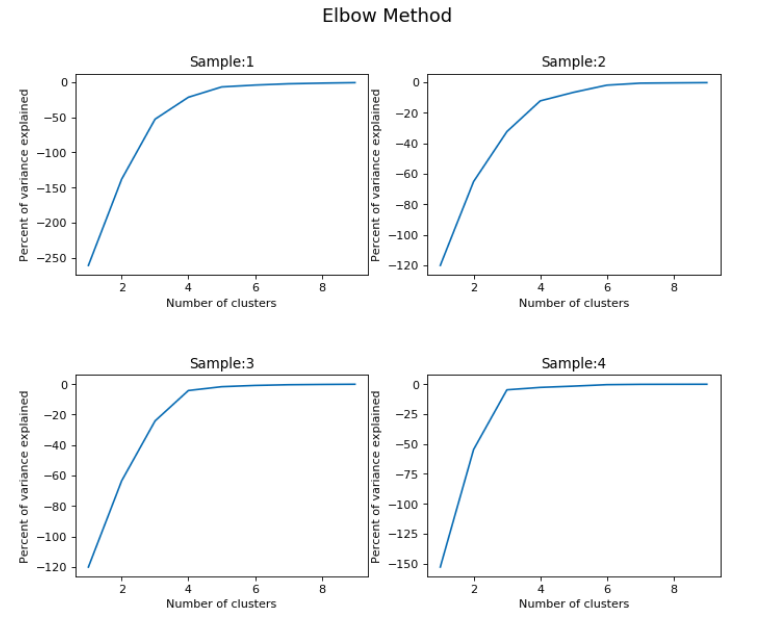
\includegraphics[width=0.90\textwidth]{elbow-method-applied.png}
\caption{Elbow method to find number of clusters}
\label{fig:elbow-method-applied}
\end{figure}

We then applied k-means++ clustering, as explained in section \ref{subsec:Clustering} on page \pageref{subsec:Clustering}, to find the correct centroids for our training examples. We found the following centroids for our training sets.

\begin{table}[H]
\centering
  \begin{tabular}{ l | c  c  c }
    Cluster      & ICMP  & TCP  & UDP \\
    \hline
    0         &{-0.16815612}       &{-0.14928111}    &{-0.16948046} \\
    1         &{-0.18181818}       &{5.13527652}     &{5.68956244} \\
    2         &{5.08663322}        &{-0.27110845}    &{-0.099885} \\
    3         &{-0.18670401}       &{-0.18804342}    &{-0.018538} \\
  \end{tabular}
\caption{Cluster centroids for our training examples} \label{table:centroids}
\end{table}

Those centroids were used for clustering our training sets. To draw the clusters in two dimensional space we had to reduce the three dimensions training example into two dimensions without losing much information. This was achieved by using Principal-Component Analysis (PCA). PCA is a technique which takes a set of tuples representing points in a high-dimensional space as input, and then finds the directions along which the tuples line up best.\cite{pca}. We used the Scikit-learn PCA module for this purpose.

\begin{figure}[H]
\centering
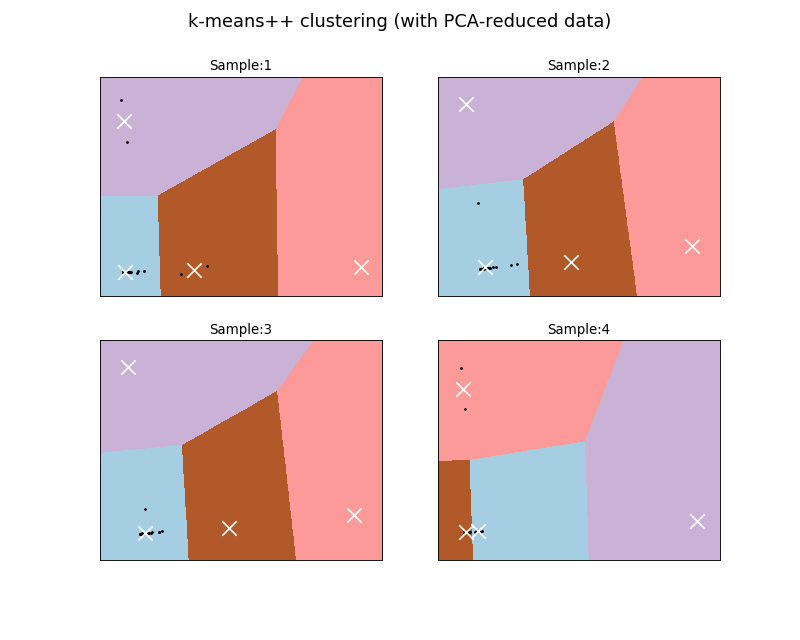
\includegraphics[width=0.90\textwidth]{kemans-clustering.png}
\caption{Clustering using k-means++ algorithm} \label{fig:k-means-clustering}
\end{figure}

The k-means++ algorithm gave a label to each training example. This label was the cluster number to which a training example was assigned. The new labeled data look like below (table \ref{table:labeled-set}).

\begin{table}[H]
\centering
  \begin{tabular}{| l | c | c | c | c |}
    \hline
    {Destination IP Address}  &ICMP  &TCP &UDP  &Cluster \\
    \hline
    172.217.10.134  & 0     & 8     & 12  &1  \\ \hline
    65.19.96.252    & 5     & 0     & 192 &0  \\ \hline
    68.67.178.134   & 0     & 78    & 0   &2  \\ \hline
  \end{tabular}
\caption{Labeled Training Set (with cluster number)} \label{table:labeled-set}
\end{table}

We also checked the clustering accuracy using the Rand Index explained in the section \ref{subsec:Clustering} on page \pageref{subsec:Clustering}. With more training sets, we observed that the RI index improves. A tag file with IP addresses, their cluster labels, and average packet count was created. This tag file was used in first pass for detecting any anomaly in the network traffic.

As explained in the section \ref{subsec:Anomaly_Detection} on page \pageref{subsec:Anomaly_Detection}, we trained the model and created the classifier for each cluster. We used Scikit-learn's OneClassSVM library to achieve this. The input vector to the classifier was the set of all the training examples belonging to the same cluster. Thus, for our four clusters, we had four classifiers. The input vector to the classifier is in the form shown in table \ref{table:labeled-set} on page \pageref{table:labeled-set}.

The following is the result of modeling on the training data sets. Each cluster has its own model. We used PCA component analysis to draw the models.

\begin{figure}[H]
\centering
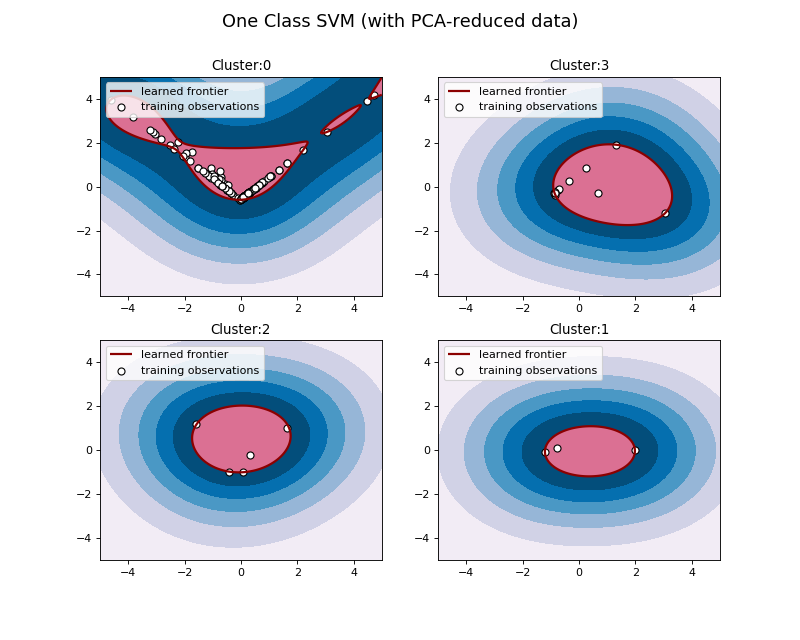
\includegraphics[width=0.80\textwidth]{one-class-SVM.png}
\caption{one-class SVM} \label{fig:one-class-SVM}
\end{figure}

At the end of the training, we had a file containing IP addresses labeled with the cluster numbers, and four classifiers for four clusters.

We applied the detection techniques explained in section \ref{sec:Detection} on page \pageref{sec:Detection} on the detection set. The detection set was created by capturing packets during the orchestrated DDoS attacks (IP address 92.168.0.7 was attacked). Using the detection techniques we were able to detect an attack on destination 92.168.0.7 in our modeled network.

\begin{figure}[H]
\centering
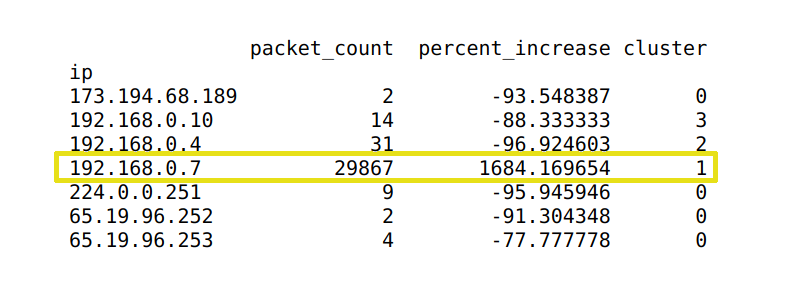
\includegraphics[width=0.80\textwidth]{detected_IP.png}
\caption{Program output} \label{fig:detected_IP}
\end{figure}

\pagebreak
\section{Mitigation}

By now we have a computer program (consisting of a few modules, i.e., clustering, classification and detection) which can run on a router and can be used to detect a DDoS attack. There are many routers through which a destination can be reached, so, to correctly detect a DDoS attack, we should have our program on every router on the Internet. We can do this, either by manually installing the program on each router, or by using Network Function Virtualization (NFV)\cite{nfv}. NFV is an advanced technology which allows us to manage network devices remotely, and also allows us to add functionality to those networking devices. Because of this virtual technology we don't have to manually install computer programs on routers; rather, we can do it any time from anywhere. Although this technology is new, it's spreading very fast, and soon it will be available for every commercial router.

After detecting an attack a router can choose to block all the packets going to the destination under attack, or it can communicate the attack information to the destination. The attack information can contain region name and packet count.

If an attack information is communicated to the destination, destination can know the nature of the attack, i.e., it can know where the attack is originated and how intense it is. Destination can also query the router for more information, such as the source IP address of the packets captured during an attack.

The control of blocking the traffic at a router can also be given to the destination. In this case, the destination can perform its own analysis, understand the nature of the attack, and then decide whether or not the incoming packets from the reporting router should be blocked. There can be different parameters based on which the destination server can decide to block the traffic. Those parameters can be provided by the router as additional information. Many questions can be asked before making the decision at a destination---such as: How many routers have reported a change in traffic, and is the attack information coming from a region which never had traffic in the past---etc.

\begin{figure}[H]
\centering
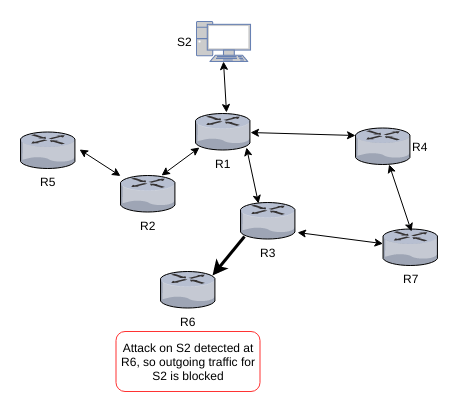
\includegraphics[scale=0.60]{mitigation_path.png}
\caption{Blocking traffic at a router: The out-bound traffic for S2 is blocked from router R6,
because attack has been detected. Traffic from all other routers is unaffected} \label{fig:mitigation_path}
\end{figure}

A router can use the existing Internet Control Message Protocol (ICMP) to communicate with a destination network. This protocol is used to provide feedback about the problems in the communication environment. ICMP messages are sent in several situations such as: 1) when a datagram cannot reach its destination; 2) when the gateway does not have the buffering capacity to forward a datagram; 3) when the gateway can direct the host to send traffic on a shorter route etc.\cite{icmp} Similarly we can use the ICMP protocol to inform the destination about the anomalies in the traffic. This protocol has many unused ``types'' (there can be 0-255 types but as of now only 0-41 are in use). We can create a new ICMP ``type'' to send DDoS attack detection information from a router to a destination server, and then the destination server can send mitigation instructions to a routers.

\begin{figure}[H]
\centering
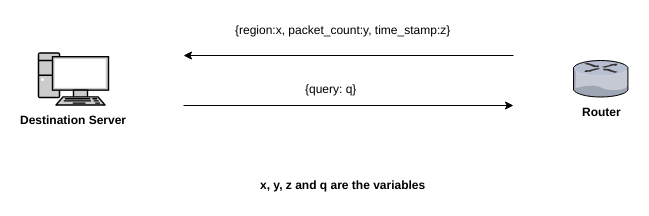
\includegraphics[scale=0.5]{router-network-communication.png}
\caption{Communication between a router and a destination server} \label{fig:router-network-communication}
\end{figure}

\pagebreak
\section{Conclusion}

DDoS attacks are a real threat to everyone on the Internet, and their detection is difficult because of the spoofing techniques employed by the attackers. We have discussed how we can combine two machine learning algorithms (clustering and classification) to efficiently detect DDoS attacks at the router. We also discussed how to create a program that uses learning algorithms, and then how to installed that program on routers. Having detection program on the routers eliminate the need for extra infrastructure for detection of a DDoS attack. With the advancement of Network Function Virtualization (NFV), it's easy to push the learning program on the routers. We also discussed how a router can stop an attack and how it can communicate the attack information with the stake holders (e.g., server) for taking better decisions about blocking the attack traffic.
\pagebreak

\singlespacing
\bibliographystyle{unsrt}   % Unsorted order
\bibliography{biblo}       % expects file "biblo.bib"

\end{document}
